\documentclass[a4paper,11pt,oneside]{book}

%%% το αρχείο αυτό καθορίζει το look που έχουν οι pythonies
%%% γίνεται \input από όλα τα κεφάλαια και τα φύλλα εργασίας

% χρησιμοποιούμενα πακέτα: 
% 
% polyglossia
% xstring
% graphicx
% caption
% xcolor
% hyperref
% minted
% geometry
% titlesec
% datetime
% changepage
% ntheorem

% οριζόμενες εντολές:
%
% smallcaps (βοηθ. removeaccents)
%    μικρά κεφαλαία χωρίς τόνους στα φωνήεντα
% scaling
%    η κλιμάκωση *όλων* των illustrations, τρέχουσα τιμή 0.9
% iconcomputer, iconkeyboard, icondiscuss, iconfillin, iconcaution, iconprompt, dottedline
%    εικονίδια για τα φύλλα εργασίας και εστιγμένη γραμμή
% marginnote
%    πλευρικό σχόλιο
% chapterwabstract (βοηθ. abstract, boxcolor, chaptercolor, concepts, tmpconcepts)
%    εισαγωγικό κείμενο κεφαλαίου με χρωματιστό τετράγωνο, συνοδευτικές έννοιες, κλπ.
% tobecontinued
%    εμφανίζει το "συνεχίζεται στην επόμενη σελίδα"

% οριζόμενα περιβάλλοντα:
% 
% note
%    μια υποσημείωση ή υπόδειξη, με μικρότερα γράμματα
% question
%    μια ερώτηση που "οδηγεί" κάθε νέα ενότητα
% answer
%    μια απάντηση σε μια ερώτηση του φύλλου εργασίας
% theory
%    μια ενότητα "θεωρίας" (στο τέλος ενός κεφαλαίου)
% exercise
%    μια αριθμημένη άσκηση
% step
%    ένα αριθμημένο βήμα (για φύλλο εργασίας)

% για μορφοποίηση κώδικα:
%
% pycode (περιβάλλον)
%     κώδικας python χωρίς αρίθμηση
% pyfile (εντολή)
%     εισαγωγή κώδικα python από αρχείο
% pyfilenl (εντολή)
%     εισαγωγή κώδικα python από αρχείο χωρίς αρίθμηση γραμμών
% pyfilesrc (εντολή)
%    εισαγωγή κώδικα από αρχείο με link στο αρχείο
% pyinline (εντολή)
%     κώδικας python μέσα στη ροή του κειμένου
% pyplain (περιβάλλον, για τα φύλλα εργασίας)
%     κώδικας python χωρίς φόντο
% pynew (περιβάλλον, για τα φύλλα εργασίας)
%     κώδικας python με φόντο
% pyterm (περιβάλλον για τα φύλλα εργασίας)
%     η είσοδος του χρήστη ή τα περιεχόμενα της οθόνης
% pyhighlight (εντολή)
%    highlight κειμένου (χρησιμοποιείται για κώδικα μέσα σε pyplain)


%%% επιλογές γλώσσας και γραμματοσειρών για το XeLaTeX

\usepackage{polyglossia}
\setdefaultlanguage{greek}
\setmainfont[Ligatures=TeX,SmallCapsFont={Linux Libertine O C},SmallCapsFeatures={Letters=SmallCaps}]{Linux Libertine O}
\setsansfont{Linux Biolinum O}
\setmonofont{Ubuntu Mono}
\enablehyphenation

% αφαίρεση τόνων από τα smallcaps
\usepackage{xstring}
\newcommand{\removeaccents}[1]{%
\def\result{#1}%
\StrSubstitute{\result}{ά}{α}[\result]%
\StrSubstitute{\result}{έ}{ε}[\result]%
\StrSubstitute{\result}{ή}{η}[\result]%
\StrSubstitute{\result}{ί}{ι}[\result]%
\StrSubstitute{\result}{ό}{ο}[\result]%
\StrSubstitute{\result}{ύ}{υ}[\result]%
\StrSubstitute{\result}{ώ}{ω}[\result]%
\StrSubstitute{\result}{Ά}{Α}[\result]%
\StrSubstitute{\result}{Έ}{Ε}[\result]%
\StrSubstitute{\result}{Ή}{Η}[\result]%
\StrSubstitute{\result}{Ί}{Ι}[\result]%
\StrSubstitute{\result}{Ό}{Ο}[\result]%
\StrSubstitute{\result}{Ύ}{Υ}[\result]%
\StrSubstitute{\result}{Ώ}{Ω}[\result]%
\result
}

\newcommand{\smallcaps}[1]{\textsc{\removeaccents{#1}}}

%%% εικόνες και λεζάντες

\usepackage{graphicx}
\newcommand{\scaling}{0.9}
\usepackage{caption}
\captionsetup{font=footnotesize}

%%% ειδικά περιβάλλοντα

\usepackage{xcolor}

% ερωτήσεις (που οδηγούν στην επόμενη ενότητα)
\definecolor{questioncolor}{rgb}{0.6,0.5,0.5}
\newenvironment{question}{\noindent\itshape\color{questioncolor}}{\noindent\ignorespaces}

% απαντήσεις (για τις ερωτήσεις των φύλλων εργασίας)
\definecolor{answercolor}{rgb}{0.5,0.5,0.5}
\newenvironment{answer}{\marginnote[16pt]{\iconfillin}\noindent\itshape\color{answercolor}}{\noindent\ignorespaces}

% περιβάλλον "θεωρίας" (πλήρες πλάτος κειμένου)
\usepackage{changepage}
\newenvironment{theory}[1]{\begin{adjustwidth}{}{-\overhang}\smallcaps{#1}\itshape}{\end{adjustwidth}}

% απομεινάρια...
% \newlength{\theoryrulelength}
% \setlength{\theoryrulelength}{36pt}
% \newenvironment{theory}{\rule{\theoryrulelength}{0.4pt}\begin{adjustwidth}{}{-\overhang}\itshape}{\end{adjustwidth}\rule{\theoryrulelength}{0.4pt}}

%%% υπερσύνδεσμοι

\definecolor{linkcolor}{rgb}{0.0,0.5,0.25}
\usepackage[colorlinks=true,urlcolor=linkcolor]{hyperref}

%%% εικονίδια και εστιγμένες γραμμές (για τα φύλλα εργασίας)

\newcommand{\iconcomputer}{
\includegraphics[scale=0.35]{../../share/circle-icons/one-color/computer.eps}}
\newcommand{\iconkeyboard}{
\includegraphics[scale=0.35]{../../share/circle-icons/one-color/keyboard.eps}}
\newcommand{\icondiscuss}{
\includegraphics[scale=0.35]{../../share/circle-icons/one-color/chat.eps}}
\newcommand{\iconfillin}{
\includegraphics[scale=0.35]{../../share/circle-icons/one-color/compose.eps}}
\newcommand{\iconcaution}{
\includegraphics[scale=0.35]{../../share/circle-icons/one-color/caution.eps}}
\newcommand{\iconprompt}{
\includegraphics[scale=0.35]{../../share/circle-icons/one-color/prompt.eps}}
\newcommand{\dottedline}{\vspace{\parskip}\dotfill}

%%% συνεχίζεται στην επόμενη σελίδα

\newcommand{\tobecontinued}{\mbox{}\hfill{\footnotesize ...συνεχίζεται στην επόμενη σελίδα.}}
\newenvironment{note}{\small\upshape}{}

%%% μορφοποίηση κώδικα με το pygmentize

\usepackage{minted}

% fix για ένα bug στο minted που εμφανίζεται όταν χρησιμοποιείται χρώμα στο φόντο (bgcolor)
% http://tex.stackexchange.com/questions/228058/how-to-space-before-and-after-a-minted-code-block-with-bgcolor
\makeatletter
\patchcmd{\minted@colorbg}{\noindent}{\noindent}{}{}
\apptocmd{\endminted@colorbg}{}{}{}
\makeatother

% χρώματα φόντου για τον κώδικα
\definecolor{codebg}{rgb}{0.80,0.95,0.85}
\definecolor{newcodebg}{rgb}{0.75,0.95,0.85}

% ορισμοί για τα περιβάλλοντα κώδικα
% pycode: περιβάλλον κώδικα python χωρίς αρίθμηση
\newminted[pycode]{python3}{bgcolor=codebg}
% pyfile: python από αρχείο
\newmintedfile[pyfile]{python3}{linenos=true,numberblanklines=false,escapeinside=||,bgcolor=codebg}
% pyfilenl: python από αρχείο χωρίς αρίθμηση γραμμών
\newmintedfile[pyfilenl]{python3}{linenos=false,numberblanklines=false,escapeinside=||,bgcolor=codebg}
% pyinline: python μέσα στη ροή του κειμένου
\newmintinline[pyinline]{python3}{linenos=true,numberblanklines=false}
% pyplain: (για τα φύλλα εργασίας) περιβάλλον χωρίς φόντο
\newminted[pyplain]{python3}{bgcolor=white,escapeinside=||,formatcom={\upshape}}
% pynew: (για τα φύλλα εργασίας) περιβάλλον με φόντο
\newminted[pynew]{python3}{bgcolor=newcodebg,escapeinside=||,formatcom={\upshape}}
% pyterm: (για τα φύλλα εργασίας) περιβάλλον για τα περιεχόμενα της οθόνης
\newminted[pyterm]{text}{bgcolor=white,escapeinside=||}

%\newminted[pyterm]{text}{escapeinside=||}
% [TODO] fix: το pyterm χωρίς bgcolor εμφανίζει μεγαλύτερα περιθώρια (πάνω και κάτω) και δεν φαίνεται ωραίο. Το bgcolor είναι προσωρινό workaround, έχει κι αυτό margins (για να μην είναι κολλητά ο κώδικας με το περιθώριο) κι έτσι ο κώδικας στ' αριστερά δεν είναι τέλεια στοιχισμένος.

% εντολή για κώδικα από αρχείο με link στο αρχείο
\newcommand{\pyfilesrc}[2][]{%
\pyfile[#1]{#2}\\
\mbox{}\hfill{\scriptsize\href{http://pythonies.mysch.gr/#2}{\url{#2}}}
}

% εντολή για το highlighting του κώδικα (συνήθως σε pyplain περιβάλλον με escapeinside)
\newcommand{\pyhighlight}[1]{\colorbox{newcodebg}{#1}}

%%% αριθμημένα περιβάλλοντα

\usepackage{ntheorem}

% άσκηση
\makeatletter
\theoremheaderfont{\upshape}%\upshape\bfseries\scshape}
\theorembodyfont{\itshape}%\slshape}
\newtheoremstyle{lmargin}%
  {\item[\theorem@headerfont \llap{##2}\hskip\labelsep\hskip-6pt]}%
  {\item[\theorem@headerfont \llap{##2}\hskip\labelsep ##1\ (##3)\theorem@separator]}
\makeatother
\theoremstyle{lmargin}
\newtheorem{exercise}{}[chapter]

% βήμα φύλλου εργασίας
\makeatletter
\theoremheaderfont{\bfseries}%\upshape\bfseries\scshape}
\theorembodyfont{\upshape}%\slshape}
\newtheoremstyle{lmarginup}%
  {\item[\theorem@headerfont \llap{##2}\hskip\labelsep\hskip-6pt]}%
  {\item[\theorem@headerfont \llap{##2}\hskip\labelsep ##1\ (##3)\theorem@separator]}
\newtheoremstyle{slmarginup}%
  {\item[\theorem@headerfont \llap{##1##2.}\hskip\labelsep\hskip-6pt]}%
  {\item[\theorem@headerfont \llap{##2.}\hskip\labelsep ##1\ (##3)\theorem@separator]}
\makeatother

% deprecated: \newcommand{\standalone}{} to define standalone
%\ifdefined\standalone
    \theoremstyle{slmarginup}
    \newtheorem{step}{}
%\else
%    \theoremstyle{lmarginup}
%    \newtheorem{step}{}[chapter]
%\fi

%%% γεωμετρία σελίδας και συναφείς ορισμοί από το tufte-latex
%%% https://tufte-latex.github.io/tufte-latex/

% εσοχή και διάστημα μεταξύ παραγράφων
% δεν επηρρεάζει το tufte-latex
\parindent=0pt
\parskip=6pt

% γεωμετρία σελίδας και ορισμός μηκών
\usepackage[a4paper,left=24.8mm,top=27.4mm,headsep=2\baselineskip,textwidth=107mm,marginparsep=8.2mm,marginparwidth=49.4mm,textheight=66\baselineskip,headheight=\baselineskip]{geometry}

\setlength{\marginparpush}{12pt}
\addtolength{\marginparpush}{\parskip}
\newlength{\fullwidth}
\setlength{\fullwidth}{\textwidth}
\addtolength{\fullwidth}{\marginparsep}
\addtolength{\fullwidth}{\marginparwidth}
\newlength{\overhang}
\setlength{\overhang}{\marginparsep}
\addtolength{\overhang}{\marginparwidth}

% απομεινάρια...
%\setlength\abovedisplayskip{6pt plus 2pt minus 4pt}
%\setlength\belowdisplayskip{6pt plus 2pt minus 4pt}

% italicize description run-in headings (instead of the default bold)
\renewcommand*\descriptionlabel[1]{\hspace\labelsep\normalfont\em #1}

% πλευρική σημείωση
\newcommand\marginnote[2][0pt]{%
  \marginpar{\hbox{}\vspace*{#1}\vspace*{-1\baselineskip}\noindent \footnotesize\textup{#2}}%
  {}%
}

% formatting title sections
\setcounter{secnumdepth}{-1}

\usepackage{titlesec}
\usepackage[nodate]{datetime}
\newlength{\beforesection}
\setlength{\beforesection}{3ex plus 0.5ex minus 0.2ex}
\addtolength{\beforesection}{-\parskip}
\newlength{\aftersection}
\setlength{\aftersection}{1.5ex plus 0.2ex}
\addtolength{\aftersection}{-\parskip}
\titlespacing*{\section}{0pt}{\beforesection}{\aftersection}

% απομεινάρια...
%\titlespacing*{\chapter}{0pt}{50pt}{40pt}
%\titlespacing*{\section}{0pt}{3.5ex plus 1ex minus .2ex}{2.3ex plus .2ex}

%%% για εισαγωγικό κείμενο κεφαλαίου με χρωματιστό τετράγωνο, συνοδευτικές έννοιες, κλπ.

\newcommand{\abstract}{}
\newcommand{\boxcolor}{}
\newcommand{\chaptercolor}{}
\newcommand{\concepts}{}
\newcommand{\tmpconcepts}{}
\newif\ifbonus

% reference: \titleformat{ command }[ shape ]{ format }{ label }{ sep }{ before-code }[ after-code ]
\titleformat{\chapter}[block]
{\Huge\sffamily}
{}
{0pt}
{\ifbonus\marginnote[-6pt]{\fcolorbox{\boxcolor}{\chaptercolor}{\makebox(40,40){\strut\textcolor{\boxcolor}{\Huge\thechapter}}}\\\vspace{\parskip}\\\tiny\today\\ \currenttime}\else\marginnote[-6pt]{\colorbox{\boxcolor}{\makebox(40,40){\strut\textcolor{\chaptercolor}{\Huge\thechapter}}}\\\vspace{\parskip}\\\tiny\today\\ \currenttime}\fi}
[\small\rmfamily\textmd\abstract\vspace{\parskip}\concepts\vspace{\parskip}\\\mbox{}\hrulefill]

\newcommand{\chapterwabstract}[5]{
	\renewcommand{\abstract}{#2}
    \renewcommand{\tmpconcepts}{#3}
	\ifdefempty{\tmpconcepts}{\renewcommand{\concepts}{}}{\renewcommand{\concepts}{\\\textbf{Έννοιες: }\tmpconcepts}}
	\renewcommand{\boxcolor}{#4}
	\renewcommand{\chaptercolor}{#5}
	\chapter{#1}
}

\definecolor{introColor}{rgb}{0.25,0.5,0.75}
\definecolor{answerColor}{rgb}{0.25,0.75,0.5}
\definecolor{crapsColor}{rgb}{0.5,0.75,0.25}
\definecolor{subtractionColor}{rgb}{0.5,0.25,0.75}
\definecolor{guessColor}{rgb}{0.75,0.25,0.5}
\definecolor{nimColor}{rgb}{0.75,0.5,0.25}
\definecolor{planetColor}{rgb}{0.25,0.25,0.75}
\definecolor{hangmanColor}{rgb}{0.25,0.75,0.25}
\definecolor{oxoColor}{rgb}{0.75,0.25,0.25}

\setcounter{part}{1}
\setcounter{chapter}{4}

%%% DOCUMENT START

\begin{document}

\chapterwabstract{Το Παιχνίδι της Αφαίρεσης}{Στο κεφάλαιο αυτό θα φτιάξουμε ένα απλό παιχνίδι δύο παικτών μ' ενδιαφέρουσα ιστορία. Στο τέλος, το πρόγραμμά μας θα συμμετέχει στο παιχνίδι, παίζοντας το ρόλο ενός από τους δύο παίκτες. Στην πορεία θα έχουμε την ευκαιρία να έρθουμε ξανά σε επαφή με τις αλγοριθμικές δομές που έχουμε συναντήσει μέχρι στιγμής, ενώ θα χρησιμοποιήσουμε \emph{υποπρογράμματα}, για να κατακερματίσουμε το πρόγραμμά μας σε απλούστερα τμήματα και να διαχειριστούμε την πολυπλοκότητά του.}{δομή επιλογής, δομή επανάληψης, υποπρογράμματα}{subtractionColor}{white}

Το παιχνίδι που θα φτιάξουμε ονομάζεται ΝΙΜ. Είναι πολύ παλιό και πιθανότατα προέρχεται από την Κίνα. Έχει πολλές παραλλαγές κι εδώ θ' ασχοληθούμε με μια απλή εκδοχή του που ονομάζεται \emph{το παιχνίδι της αφαίρεσης}. Ένα πλήθος από αντικείμενα (π.χ. σπίρτα, ξυλάκια) τοποθετούνται στη σειρά και ο κάθε ένας από τους δύο παίκτες αφαιρεί με τη σειρά του από ένα μέχρι και τρία αντικείμενα, μέχρι να μείνει μόνο ένα. Ο παίκτης που θα μείνει με το τελευταίο αντικείμενο όταν είναι η σειρά του να παίξει \emph{χάνει} το παιχνίδι. Στη γενικότερη εκδοχή του ΝΙΜ, υπάρχουν περισσότερες σειρές από αντικείμενα.

Το ΝΙΜ είναι ένα από τα πρώτα παιχνίδια που αυτοματοποιήθηκαν και, όπως θα δούμε στη συνέχεια, υπάρχει λόγος γι' αυτό. Ήδη από το 1940 η αμερικάνικη εταιρεία Westinghouse παρουσίασε ένα μηχάνημα που έπαιζε ΝΙΜ, το Nimatron, ενώ στις αρχές της δεκαετίας του '50 εμφανίστηκαν ειδικού σκοπού ηλεκτρονικοί υπολογιστές που έπαιζαν ΝΙΜ, όπως ο NIMROD της βρετανικής Ferranti.

%%%%%%%%

\section{Το Στήσιμο}

\begin{question}
Ας υποθέσουμε ότι τα αντικείμενα που χρησιμοποιούν οι παίκτες είναι σπίρτα. Με πόσα πρέπει να ξεκινήσουμε;
\end{question}

Οι κανόνες του παιχνιδιού δεν προσδιορίζουν το αρχικό πλήθος των σπίρτων. Μπορούμε λοιπόν να το ορίσουμε μόνοι μας.

\begin{pycode}
# αρχικό πλήθος σπίρτων
matches = 7
\end{pycode}

Εναλλακτικά, μπορούμε να αρχικοποιήσουμε την μεταβλητή \pyinline{matches} με μια τυχαία τιμή (ας πούμε από το 7 μέχρι και το 21).

%\marginnote[18pt]{Η βιβλιοθήκη \pyinline{random} περιέχει συναρτήσεις για την παραγωγή τυχαίων αριθμών. Για να τη χρησιμοποιήσουμε θα πρέπει να την εισάγουμε (\pyinline{import}).}
%\marginnote{Η συνάρτηση \pyinline{randint()} από τη βιβλιοθήκη \pyinline{random}, παράγει τυχαίους ακέραιους αριθμούς, μέσα στα όρια που ορίζουν οι παράμετροί της.}
\pyfile[firstline=1,lastline=3]{src/nim.1.py}

%Η απόδοση αρχικής τιμής σε μια μεταβλητή, όπως έγινε εδώ για την μεταβλητή \pyinline{matches}, ονομάζεται \emph{αρχικοποίηση}. Κατά τη διάρκεια του παιχνιδιού, καθώς οι παίκτες αφαιρούν σπίρτα, η τιμή της \pyinline{matches} θα τροποποιηθεί, όμως η αρχική τιμή καθορίζει το σημείο εκκίνησης.

Καλό θα ήταν να ενημερώσουμε το χρήστη με ένα κατάλληλο μήνυμα για τον αρχικό αριθμό των σπίρτων.

\pyfile[firstline=4,lastline=5]{src/nim.1.py}

%%%%%%%%

\section{Κάνε Ένα Γύρο}

\begin{question}
Τώρα θα πρέπει να γράψω τις εντολές για έναν γύρο του παιχνιδιού και να τις κάνω να επαναλαμβάνονται μέχρι να τελειώσει το παιχνίδι.
\end{question}

Το συγκεκριμένο παιχνίδι συνεχίζεται όσο τα σπίρτα που απομένουν είναι περισσότερα του ενός -- αυτή είναι και η \emph{συνθήκη συνέχειας} της επανάληψης.

\pyfile[firstline=6,lastline=7]{src/nim.1.py}

Θα ακολουθήσουν οι εντολές που είναι εμφωλευμένες στην επαναληπτική δομή, δηλαδή οι εντολές που θα πρέπει να εκτελούνται ξανά και ξανά σε κάθε γύρο του παιχνιδιού.

%Η συνθήκη συνέχειας της επανάληψης %\pyinline{matches > 1}
%ελέγχεται \emph{πριν} από κάθε κύκλο για να διαπιστωθεί αν η επανάληψη πρέπει να συνεχιστεί. Όταν διαπιστωθεί ότι η συνθήκη δεν ισχύει (είναι \emph{ψευδής}), η επανάληψη τερματίζεται. Σημειώστε ότι η συνθήκη μπορεί να μην ισχύει ήδη από την πρώτη φορά που θα ελεγχθεί, οπότε σε αυτή την περίπτωση οι εντολές της επανάληψης δεν θα εκτελεστούν ούτε μία φορά.

Σε κάθε γύρο θα ζητείται από έναν παίκτη το πλήθος των σπίρτων που επιθυμεί να αφαιρέσει. 
%Στην μεταβλητή \pyinline{removed} αποθηκεύεται το πλήθος των σπίρτων που πληκτρολογεί ο παίκτης. 

\marginnote[18pt]{Η τιμή που επιστρέφει η \pyinline{input()} είναι \emph{αλφαριθμητική}, πρόκειται για το κείμενο που πληκτρολόγησε ο χρήστης. Χρειάζεται να μετατρέψουμε την τιμή αυτή σε ακέραιο αριθμό, να της αλλάξουμε τον \emph{τύπο}, και για την μετατροπή αυτή χρησιμοποιούμε την \pyinline{int()}.}
\pyfile[firstline=8,lastline=10]{src/nim.1.py}

Η μεταβλητή \pyinline{matches} θα πρέπει να μειώνεται σε κάθε κύκλο κατά το πλήθος των σπίρτων που αφαιρούνται από το τραπέζι.

\pyfile[firstline=11,lastline=12]{src/nim.1.py}

Κάτι ακόμα που χρειάζεται σε κάθε κύκλο του παιχνιδιού είναι να εμφανίζουμε στους παίκτες την τιμή της μεταβλητής \pyinline{matches}, ώστε να αποφασίζουν για το πλήθος των σπίρτων που θα αφαιρέσουν.

\pyfilesrc[firstline=13,lastline=14]{src/nim.1.py}

%%%%%%%%

\section{Ποιός Παίζει;}

\begin{question}
Προς το παρόν δεν υπάρχει διαφοροποίηση ανάμεσα στους παίκτες. Δεν ξέρουμε ούτε ποιος παίζει κάθε φορά, ούτε ποιος νικάει.
\end{question}

Σε κάθε κύκλο του παιχνιδιού, το πρόγραμμα ρωτάει πόσα σπίρτα θα αφαιρεθούν. Ωστόσο, δεν καταγράφει ποιος από τους δύο παίκτες είναι που αφαιρεί κάθε φορά τα σπίρτα κι έτσι δεν είναι σε θέση να υπολογίσει ποιος είναι ο νικητής όταν απομείνει μόνο ένα. 

Υπάρχουν αρκετοί τρόποι να λύσουμε αυτό το πρόβλημα. Μια απλή προσέγγιση είναι να χρησιμοποιήσουμε μια μεταβλητή \pyinline{player}, η οποία σε κάθε γύρο θα παίρνει \emph{εναλλάξ} την τιμή 1 ή 2, υποδεικνύοντας με αυτόν τον τρόπο ποιος παίκτης έχει σειρά να παίξει.

Αρχικά, πριν ξεκινήσει η διαδικασία του παιχνιδιού, ορίζουμε ποιος παίκτης θα ξεκινά πρώτος. Αυτό δεν πρόκειται να αλλάξει -- πρώτος θα ξεκινά πάντα ο παίκτης με αριθμό \pyinline{1}.

\pyfile[firstline=6,lastline=7]{src/nim.2.py}

Τώρα πλέον η προτροπή που εμφανίζεται σε κάθε κύκλο απευθύνεται σε συγκεκριμένο παίκτη:

\pyfilesrc[firstline=10,lastline=12]{src/nim.2.py}

Στο τέλος κάθε κύκλου της επανάληψης, η τιμή της μεταβλητής \pyinline{player} θα πρέπει να τροποποιείται, ώστε να υποδεικνύει τον επόμενο παίκτη που έχει σειρά να παίξει. %εναλλάσσεται από το 1 στο 2 και αντίστροφα. 
Θα χρειαστούμε ένα υποπρόγραμμα, το οποίο θα δέχεται σαν παράμετρο τον αριθμό ενός παίκτη και θα επιστρέφει τον αριθμό του επόμενου παίκτη. 

\pyfile[firstline=2,lastline=10]{src/nim.3.py}

Υπάρχουν κι άλλοι τρόποι να επιτευχθεί το ίδιο αποτέλεσμα, όπως φαίνεται στην εναλλακτική υλοποίηση που ακολουθεί. Ωστόσο, ο τρόπος που λειτουργεί η συνάρτηση δεν έχει σημασία για εκείνους που την καλούν.

\marginnote[18pt]{Η έκφραση \pyinline{p}\%2 υπολογίζει το υπόλοιπο της ακέραιας διαίρεσης του \pyinline{p} με το \pyinline{2}. Η τιμή της μπορεί να είναι 0 ή 1.}
\begin{pycode}
def next(p):
    """ Επιστρέφει τον αριθμό του παίκτη
    που παίζει μετά τον παίκτη p.
    p: αριθμός παίκτη (1 ή 2)
    """
    return (p % 2) + 1
\end{pycode}

Στο κύριο πρόγραμμα, στο τέλος της επανάληψης, η επόμενη τιμή της μεταβλητής \pyinline{player} είναι ο αριθμός του επόμενου παίκτη, %δηλαδή η τιμή που επιστρέφει η συνάρτηση \pyinline{nextPlayer()}.

\pyfile[firstline=26,lastline=27]{src/nim.3.py}

Όταν η επανάληψη τελειώσει, η μεταβλητή \pyinline{player} δείχνει ποιος παίκτης είχε σειρά να παίξει όταν απέμεινε ένα σπίρτο. Συνεπώς, μπορούμε να χρησιμοποιήσουμε την μεταβλητή \pyinline{player} για να διαπιστώσουμε ποιος παίκτης έχασε.

\marginnote[18pt]{Δεν υπάρχει εσοχή πριν από αυτή την εντολή, είναι στοιχισμένη πιο αριστερά από τις προηγούμενες. Αυτό υποδηλώνει ότι δεν ανήκει στην επανάληψη, αντίθετα είναι η πρώτη εντολή που θα εκτελεστεί όταν η επανάληψη διακοπεί.}
\pyfilesrc[firstline=28,lastline=29]{src/nim.3.py}

%%%%%%%%

\section{Μη Λέμε κι Ό,τι Θέλουμε}

\begin{question}
Το πρόγραμμά μας επιτρέπει στους παίκτες να αφαιρέσουν σ' έναν γύρο όσα σπίρτα θέλουν! 
%Περισσότερα από τρία και περισσότερα κι απ' όσα έχουν απομείνει στο τραπέζι.
\end{question}

Σύμφωνα με τους κανόνες του παιχνιδιού, ένας παίκτης επιτρέπεται να αφαιρέσει από ένα μέχρι και τρία σπίρτα κάθε φορά, αρκεί τα σπίρτα που έχουν απομείνει στο τραπέζι να είναι περισσότερα από τρία. Σε διαφορετική περίπτωση, θα πρέπει να αφήσει στο τραπέζι τουλάχιστον ένα σπίρτο. 

Θα φτιάξουμε ένα υποπρόγραμμα που δέχεται σαν παράμετρο το πλήθος των σπίρτων που έχουν απομείνει κι επιστρέφει το \emph{μέγιστο} πλήθος σπίρτων που επιτρέπεται ν' αφαιρεθούν. Χρειαζόμαστε αυτό το άνω όριο, για να μπορούμε να ελέγξουμε παρακάτω αν το πλήθος των σπίρτων που επιθυμεί ν' αφαιρέσει ο παίκτης είναι έγκυρο. 

\pyfile[firstline=11,lastline=20]{src/nim.4.py}

Τώρα μπορούμε να κατασκευάσουμε ένα υποπρόγραμμα το οποίο διαβάζει από τον παίκτη το πλήθος των σπίρτων που επιθυμεί να αφαιρέσει. Το υποπρόγραμμα \emph{ελέγχει} την τιμή που δίνει ο παίκτης και \emph{εξασφαλίζει} ότι αυτή δεν παραβιάζει τους κανόνες του παιχνιδιού. Όσο το πλήθος που πληκτρολογείται δεν είναι έγκυρο, η ανάγνωση τιμής επαναλαμβάνεται. Το υποπρόγραμμα δέχεται ως παραμέτρους τον αριθμό του παίκτη που έχει σειρά να παίξει (για να εμφανίσει την κατάλληλη προτροπή) και το πλήθος των σπίρτων που απομένουν (για να κάνει τους απαραίτητους ελέγχους).

\pyfile[firstline=21,lastline=41]{src/nim.4.py}

Τώρα, στο κύριο πρόγραμμα δεν διαβάζουμε απευθείας το πλήθος το σπίρτων, αλλά καλούμε το υποπρόγραμμα για αυτή τη δουλειά. 

\pyfilesrc[firstline=52,lastline=53]{src/nim.4.py}

%Το υποπρόγραμμα \pyinline{readMatches()} μπορεί να υλοποιηθεί με πολλούς διαφορετικούς τρόπους. Είναι όμως σημαντικό ότι οποιαδήποτε αλλαγή στη \pyinline{readMatches()} δεν αφορά το υπόλοιπο πρόγραμμα. 

%\pyfile[firstline=11,lastline=31]{src/nim.4.break.py}

%Δεν είναι φρόνιμο να κάνουμε αυτές τις προσθήκες επιτόπου, γιατί θα αυξηθεί σημαντικά η έκταση και η πολυπλοκότητα του κώδικα. Η ενδεδειγμένη προσέγγιση είναι να φτιάξουμε ένα υποπρόγραμμα το οποίο θα υλοποιεί την συγκεκριμένη λειτουργία: να ζητά από τους παίκτες το πλήθος των σπίρτων που επιθυμούν να αφαιρέσουν. Όσο περίπλοκο κι αν είναι το υποπρόγραμμα, το σημείο στο οποίο καλείται θα παραμείνει απλό και κατανοητό.

%Στην πρώτη του εκδοχή, το υποπρόγραμμα θα λειτουργεί χωρίς ελέγχους. Η παράμετρος \pyinline{p} είναι απαραίτητη για την εμφάνιση της προτροπής προς τον παίκτη.

%\pyfile[firstline=2,lastline=11]{src/nim.3.py}

%\pyfile[firstline=20,lastline=21]{src/nim.3.py}

%%%%%%%%

\section{Χαζό Μηχάνημα}

\begin{question}
Βαριέμαι να παίζω μόνος μου. Δεν γίνεται να παίζω με αντίπαλο το πρόγραμμά μου;
\end{question}

Το πρόγραμμά μας θα πρέπει να αποφασίζει για το πλήθος των σπίρτων που θα αφαιρέσει. Δεν είναι ανάγκη να καταλήξουμε από την αρχή σε κάποια ευφυή στρατηγική, μπορούμε να ξεκινήσουμε με μια τυχαία επιλογή σπίρτων. 

Θα κατασκευάσουμε ένα απλό υποπρόγραμμα το οποίο δέχεται σαν παράμετρο το πλήθος των σπίρτων που έχουν απομείνει και επιλέγει τυχαία να αφαιρέσει από \pyinline{1} μέχρι το μέγιστο πλήθος σπίρτων που επιτρέπεται να αφαιρεθούν.

\marginnote[18pt]{Οι παράμετροι που χρησιμοποιούνται κατά την κλήση μιας συνάρτησης δεν είναι μόνο σταθερές ή μεταβλητές, αλλά κι ολόκληρες εκφράσεις, που μπορεί να περιλαμβάνουν και κλήσεις συναρτήσεων. Πρώτα υπολογίζεται η τιμή κάθε παραμέτρου και μετά ενεργοποιείται η εκτέλεση των εντολών της συνάρτησης που καλείται.}
\pyfile[firstline=42,lastline=47]{src/nim.5.py}
\clearpage

Στην τελευταία γραμμή, η τιμή που επιστρέφει η \pyinline{maxMatches()} χρησιμοποιείται ως άνω όριο για τον τυχαίο αριθμό που θα δημιουργηθεί. Είναι σχεδόν το ίδιο με τον κώδικα που ακολουθεί, αλλά χωρίς την ενδιάμεση μεταβλητή \pyinline{limit}.

\begin{pycode}
    limit = maxMatches(m)
    return random.randint(1,limit)
\end{pycode}

Είναι ενδιαφέρον ότι η συνάρτηση \pyinline{maxMatches()} χρησιμοποιείται τώρα και από την \pyinline{readMatches()} για την ανάγνωση αριθμού από τον χρήστη, αλλά και από την \pyinline{randomMatches()} για την επιλογή ενός αριθμού σπίρτων από το ίδιο το πρόγραμμα.

Ας εστιάσουμε τώρα στο κύριο πρόγραμμα. Θα χρησιμοποιήσουμε μια μεταβλητή \pyinline{computer}, η οποία στην αρχή του παιχνιδιού παίρνει τυχαία την τιμή \pyinline{1} ή \pyinline{2}. Γνωρίζουμε έτσι ποιος από τους δύο παίκτες παίζει πλέον αυτοματοποιημένα, ενώ αποφασίζεται τυχαία αν ξεκινά πρώτος ή δεύτερος. 

\pyfile[firstline=52,lastline=53]{src/nim.5.py}

Θυμηθείτε ότι στο τέλος κάθε γύρου, η μεταβλητή \pyinline{player} εναλλάσσεται μεταξύ των τιμών \pyinline{1} και \pyinline{2}, υποδεικνύοντας ποιος παίκτης έχει σειρά να παίξει στον επόμενο γύρο. Τώρα λοιπόν θα πρέπει να ελέγχουμε αν ο επόμενος παίκτης είναι ο άνθρωπος ή το πρόγραμμά μας, ώστε να καλέσουμε σε κάθε περίπτωση την ανάλογη συνάρτηση που θα μας επιστρέψει το πλήθος των σπίρτων που θα αφαιρεθούν.

\pyfile[firstline=58,lastline=65]{src/nim.5.py}

Χρειάζεται να φροντίσουμε μια ακόμα σημαντική λεπτομέρεια. Μέχρι στιγμής, στο τέλος του παιχνιδιού ανακοινώνεται ο \emph{αριθμός} του παίκτη που έχασε. Τώρα που μόνο ο ένας παίκτης είναι άνθρωπος, είναι προτιμότερο να εμφανίζουμε διαφοροποιημένα μηνύματα.

\pyfilesrc[firstline=73,lastline=77]{src/nim.5.py}

%%%%%%%%

\section{Άνθρωπος Εναντίον Μηχανής}

\begin{question}
Όταν το πρόγραμμά μου παίζει τυχαία δεν έχει και μεγάλο ενδιαφέρον. Δεν γίνεται να το κάνουμε λίγο πιο ``έξυπνο'';
\end{question} 

Θα πρέπει πρώτα εμείς να σχεδιάσουμε έναν καλύτερο τρόπο παιχνιδιού και μετά να τον περιγράψουμε με τις κατάλληλες εντολές.
%
\marginnote{\begin{center}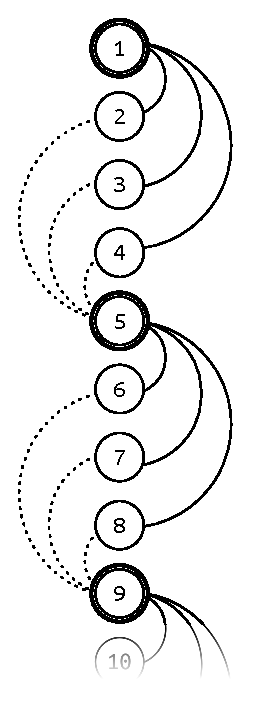
\includegraphics[scale=\scaling]{illustrations/strategy.eps}\end{center}
Οι κύκλοι αντιστοιχούν στις διαφορετικές καταστάσεις του παιχνιδιού: ο αριθμός κάθε κύκλου είναι τα σπίρτα που απομένουν σε κάθε κατάσταση.
Οι καταστάσεις 1, 5, 9, ... είναι οι «ανεπιθύμητες νησίδες»: όταν ένας παίκτης βρίσκεται σε μια από αυτές τότε ο αντίπαλός του μπορεί πάντα να τον οδηγήσει στην επόμενη νησίδα και, τελικά, στην ήττα.}
Είναι ευκολότερο ν' αρχίσουμε μελετώντας ποιες είναι οι ενδεδειγμένες κινήσεις όταν απομένουν 2, 3 ή 4 σπίρτα: ο παίκτης που έχει σειρά να παίξει μπορεί να αφαιρέσει αντίστοιχα 1, 2 ή 3 σπίρτα και να κερδίσει άμεσα. Αντίθετα, όταν απομένουν 5 σπίρτα η κατάσταση είναι δύσκολη: όσα σπίρτα και να αφαιρέσει ο παίκτης που έχει σειρά να παίξει, η έκβαση είναι στα χέρια του αντιπάλου. 

Ανάλογες δυσάρεστες καταστάσεις, που θα ονομάσουμε «ανεπιθύμητες νησίδες», αντιμετωπίζει ο παίκτης που έχει σειρά να παίξει όταν απομένουν 9, 13, 17, κ.ο.κ σπίρτα. Όσα σπίρτα κι αν αφαιρέσει, ο αντίπαλος μπορεί να τον στείλει στην επόμενη νησίδα.

Με βάση τα παραπάνω, παρατηρώντας ότι κάθε ανεπιθύμητη νησίδα διαφέρει από την επόμενη κατά 4 σπίρτα, μπορούμε να υλοποιήσουμε ένα υποπρόγραμμα που δέχεται σαν παράμετρο το πλήθος των σπίρτων που απομένουν και επιστρέφει το πλήθος των σπίρτων που πρέπει να αφαιρεθούν ώστε ο αντίπαλος να οδηγηθεί σε μια ανεπιθύμητη νησίδα. Στην περίπτωση που ο παίκτης βρίσκεται ήδη σε ανεπιθύμητη νησίδα, επιστρέφεται ένας τυχαίος αριθμός σπίρτων, καλώντας την \pyinline{randomMatches()}. 

\begin{pycode}
def computeMatches(m):
    """ Επιλέγει κι επιστρέφει το βέλτιστο
    πλήθος σπίρτων που θα πρέπει να αφαιρεθούν. 
    Αν δεν υπάρχει, επιστρέφει μια τυχαία τιμή.
    m: πλήθος σπίρτων που απομένουν
    """
    # υπολογισμός υπολοίπου
    mod = m % 4
    if mod == 0:
        return 3
    elif mod == 1:
        # ανεπιθύμητη νησίδα: τυχαία κίνηση
        return randomMatches(m)
    elif mod == 2:
        return 1  
    else:
        return 2
\end{pycode}

Υπάρχει και αμεσότερος τρόπος να υπολογίσει κανείς το βέλτιστο πλήθος των σπίρτων που πρέπει να αφαιρεθούν.
Σε μια ανεπιθύμητη νησίδα ισχύει ότι αν αφαιρέσεις από το πλήθος των σπίρτων μια μονάδα, τότε αυτό διαιρείται ακριβώς με το 4. Αν \emph{δεν} ισχύει αυτό, τότε η διαίρεση με το 4 έχει κάποιο \emph{υπόλοιπο} και αυτό ακριβώς το υπόλοιπο είναι τo πλήθος των σπίρτων που πρέπει να αφαιρεθούν για να οδηγήσεις τον αντίπαλό σου σε μια νησίδα.

\pyfile[firstline=48,lastline=61]{src/nim.6.py}

Στο κύριο πρόγραμμα, η κλήση της \pyinline{randomMatches()} για την επιλογή ενός τυχαίου πλήθους σπίρτων πρέπει τώρα να αντικατασταθεί από την κλήση της \pyinline{computeMatches()}. %Είναι βέβαια ενδιαφέρον ότι η τελευταία ίσως χρειαστεί και η ίδια να καλέσει την \pyinline{randomMatches()}, εφόσον το πρόγραμμά μας βρεθεί σε ανεπιθύμητη νησίδα.

\pyfilesrc[firstline=74,lastline=76]{src/nim.6.py}

%%%%%%%%

\section{Πλήρες Τελικό Πρόγραμμα}

\pyfile[firstline=1,lastline=22]{src/nim.final.py}
\tobecontinued

\pyfile[firstline=24,firstnumber=21,lastline=66]{src/nim.final.py}
\tobecontinued

\pyfilesrc[firstline=68,firstnumber=62]{src/nim.final.py}

%%%%%%%%

\section{Τροποποιήσεις -- Επεκτάσεις}

\begin{exercise}
Να υλοποιήσετε την συνάρτηση \pyinline{readMatches()} χρησιμοποιώντας μόνο την \pyinline{break} για να διακόψετε τον επαναληπτικό έλεγχο. Η συνθήκη συνέχειας της \pyinline{while} θα πρέπει να είναι η \pyinline{True}.
\end{exercise}

\begin{exercise}
Να υλοποιήσετε μια συνάρτηση η οποία ανακοινώνει το νικητή του παιχνιδιού, αφού δεχτεί τις κατάλληλες παραμέτρους. Χρησιμοποιήστε την συνάρτησή σας καλώντας την από το κύριο πρόγραμμα.
\end{exercise}

\begin{exercise}
Να τροποποιήσετε το παιχνίδι έτσι ώστε ο παίκτης που παίρνει τα τελευταία σπίρτα να κερδίζει. Ποιά είναι τώρα η βέλτιση στρατηγική για έναν παίκτη; Τροποποιήστε ανάλογα την συνάρτηση \pyinline{computeMatches()} που υπολογίζει τον αριθμό σπίρτων που πρέπει ν' αφαιρεθούν σε μια δεδομένη κατάσταση.
\end{exercise}

% άσκηση: να διαβαζονται τα ονόματα των παικτών
% άσκηση: συνάρτηση για να ανακοινώνεται ποιος ξεκινάει πρώτος. 

%\begin{exercise}
%Να επεκτείνετε το πρόγραμμα έτσι ώστε να ζητούνται τα ονόματα των δύο παικτών. Τώρα όλα τα μηνύματα που απευθύνονται στους παίκτες θα πρέπει να χρησιμοποιούν τα ονόματα αυτά, αντί του αριθμού κάθε παίκτη.
%\end{exercise}

\section{Ασκήσεις}

\begin{exercise}
Να επεκτείνετε το παιχνίδι Ανάμεσα ή Acey Ducey (κεφ. 2), έτσι ώστε να παίζεται επαναληπτικά. Το πρόγραμμά σας θα πρέπει αρχικά να ρωτάει τον παίκτη το συνολικό ποσό με το οποίο επιθυμεί να ξεκινήσει το παιχνίδι. Με το ίδιο ακριβώς ποσό θα ξεκινήσει και η «μάνα». Σε κάθε γύρο, όταν ο παίκτης ερωτάται για το ποσό που θα στοιχηματίσει, το πρόγραμμά σας θα πρέπει να ελέγχει ότι το ποσό αυτό είναι θετικό και δεν ξεπερνά το συνολικό ποσό που διαθέτει \emph{εκείνη την στιγμή} ο παίκτης, διαφορετικά θα πρέπει να επαναλαμβάνει την ερώτηση μέχρι το στοίχημα να είναι έγκυρο. Το παιχνίδι θα τελειώνει όταν εξαντληθούν τα χρήματα του παίκτη ή της «μάνας». 
%\begin{note}
%Αν η «μάνα» δεν έχει επαρκή χρήματα για να πληρώσει τον παίκτη τότε του δίνει όσα έχει (και φυσικά τερματίζεται το παιχνίδι).
%\end{note} 
\end{exercise}

\begin{exercise}
Στο παιχνίδι «Τα Ζυγά Κερδίζουν» οι δύο παίκτες ξεκινούν με μια σειρά από αντικείμενα. Το αρχικό πλήθος των αντικειμένων πρέπει να είναι περιττός αριθμός. Κάθε ένας από τους δύο παίκτες αφαιρεί με τη σειρά του από ένα μέχρι και τέσσερα αντικείμενα, μέχρι ν' αφαιρεθούν όλα. Νικητής είναι ο παίκτης που στο τέλος του παιχνιδιού απομένει με άρτιο (ζυγό) πλήθος αντικειμένων. Να αναπτύξετε ένα πρόγραμμα που θα διαβάζει σε κάθε γύρο τον αριθμό των σπίρτων που αφαιρεί ο παίκτης που έχει σειρά και στο τέλος ανακοινώνει το νικητή.
\end{exercise}

\begin{exercise}
Στο παιχνίδι «Τα Ζυγά Κερδίζουν» υπάρχουν επίσης ανεπιθύμητες νησίδες, δηλαδή καταστάσεις από τις οποίες ένας παίκτης δεν μπορεί ν' αποφύγει την ήττα, εφόσον ο αντίπαλός του παίξει σωστά. Αν ένας παίκτης δεν βρίσκεται σε ανεπιθύμητη νησίδα τότε μπορεί να οδηγήσει τον αντίπαλό του σε μία και να κερδίσει. Προσπαθήστε να καταγράψετε τις πιθανές καταστάσεις του παιχνιδιού όταν απομένουν λίγα σπίρτα (π.χ. από 1 μέχρι και 6) και ποια είναι η καλύτερη κίνηση σε κάθε μία απ' αυτές. Το εγχείρημα είναι δυσκολότερο απ' ότι στο Παιχνίδι της Αφαίρεσης γιατί εδώ η καλύτερη κίνηση δεν εξαρτάται μόνο από το πλήθος των σπίρτων που απομένουν. Πρέπει να λάβετε υπόψη αν ο καθένας από τους δύο παίκτες έχει συγκεντρώσει άρτιο ή περιττό πλήθος σπίρτων. Τελικός σας σκοπός είναι να τροποποιήσετε το πρόγραμμα της προηγούμενης άσκησης έτσι ώστε να παίζει με αντίπαλο το χρήστη.
\end{exercise}


\begin{exercise}
Τα παιδιά στο δημοτικό μαθαίνουν πρόσθεση μέσα από ασκήσεις αυξανόμενης δυσκολίας. Αρχικά, τους ζητείται να προσθέσουν δύο μονοψήφιους αριθμούς, το άθροισμα των οποίων δεν ξεπερνά το 9. 

\begin{note}
Παράδειγμα: 4 + 2 = \_
\end{note}

%Στη συνέχεια, μαθαίνουν τα «ζευγαράκια του 10», τους δίνεται δηλαδή ένας μονοψήφιος αριθμός και τους ζητείται ένας δεύτερος έτσι ώστε το άθροισμά τους να ισούται με 10. 

%{\small\upshape Παράδειγμα: 4 + \_ = 10}

Μετά τους ζητείται να προσθέσουν δύο μονοψήφιους αριθμούς, το άθροισμα των οποίων ξεπερνά το 10. 

\begin{note}
Παράδειγμα: 4 + 8 = \_
\end{note}

Το επόμενο στάδιο είναι η πρόσθεση ενός διψήφιου κι ενός μονοψήφιου, το άθροισμα των οποίων πιθανώς να ξεπερνά τη δεκάδα του διψήφιου, αλλά όχι το 99.

\begin{note}
Παράδειγμα: 42 + 9 = \_
\end{note}

Μπορείτε να φτιάξετε ένα πρόγραμμα εξάσκησης για τα παιδιά του Δημοτικού. Αρχικά, το πρόγραμμά σας θα πρέπει να ρωτά ποιο είναι το επιθυμητό επίπεδο ασκήσεων και να παράγει πέντε από αυτές. Εδώ έχουμε περιγράψει τα τρία πρώτα επίπεδα, αλλά εσείς μπορείτε να φτιάξετε κι άλλα ή ακόμα και να περάσετε σε άλλες πράξεις εκτός από την πρόσθεση. Μην σας απασχολεί αν καμιά φορά τυχαίνει να εμφανίζονται διπλότυπες ασκήσεις, αυτό προς το παρόν είναι δύσκολο να το αποφύγετε. Αν το παιδί κάνει λάθος σε κάποια από τις ερωτήσεις το πρόγραμμα μπορεί να του εμφανίζει άμεσα την σωστή απάντηση ή να του δίνει κι άλλες ευκαιρίες. Ακόμα καλύτερο θα ήταν αν το πρόγραμμά σας εξηγούσε πως προκύπτει η σωστή απάντηση ή έδινε μια υπόδειξη πριν το παιδί ξαναπροσπαθήσει.

\begin{note}
Παράδειγμα: 42 + 9 = \_. Το παιδί πληκτρολογεί 52 και το πρόγραμμα του ζητά να ξαναπροσπαθήσει, υποδεικνύοντας ότι 42 + 9 = 42 + 8 + 1 = \_
\end{note}
\end{exercise}

%%%%%%%%

\section*{}
\vspace{4\parskip}
\hrulefill

\begin{theory}{Υποπρογράμματα}
Είδαμε ήδη ότι για να αντιμετωπίσουμε την αυξανόμενη έκταση και πολυπλοκότητα των προγραμμάτων χρησιμοποιούμε \emph{υποπρογράμματα}, μικρά προγράμματα που τα συνδυάζουμε για να φτιάξουμε συνθετότερα, κατά τον ίδιο τρόπο με τον οποίο κατασκευάζουμε μια περίπλοκη μηχανή από απλούστερα εξαρτήματα, κάθε ένα από τα οποία εξυπηρετεί μια συγκεκριμένη λειτουργία. Ο κατακερματισμός των προγραμμάτων σε απλούστερα μας βοηθά να σκεφτόμαστε τμηματικά και να αναλύουμε το γενικότερο πρόβλημα σε επιμέρους απλούστερα προβλήματα. Τα υποπρογράμματα θα πρέπει να θεωρούνται όσο το δυνατόν ανεξάρτητα από το πλαίσιο μέσα στο οποίο χρησιμοποιούνται. Αντιμετωπίζουμε κάθε υποπρόγραμμα ως ένα κομμάτι κώδικα που λύνει ένα μικρό πρόβλημα με γενικό τρόπο και έτσι είναι \emph{επαναχρησιμοποιήσιμο}. Μπορεί να κληθεί από διαφορετικά σημεία και για διαφορετικούς λόγους μέσα σ' ένα πρόγραμμα, αλλά και να χρησιμοποιηθεί και σε άλλα προγράμματα στο μέλλον. 
%Λόγω ανεξαρτησίας και μικρού μεγέθους, είναι επίσης ευκολότερο να \emph{ελεγχθεί} η ορθότητα της λειτουργίας ενός υποπρογράμματος
Οι εσωτερικές λεπτομέρειες της λειτουργίας κάθε υποπρογράμματος είναι κρυμμένες για εκείνους που το χρησιμοποιούν. Όποιος θέλει να χρησιμοποιήσει ένα υποπρόγραμμα δεν χρειάζεται να καταλαβαίνει πως λειτουργεί και με ποια μέθοδο υπολογίζεται το αποτέλεσμα. Ο Al Sweigart, στο εξαιρετικό του βιβλίο Invent Your Own Computer Games with Python, γράφει: «Το ωραίο με τις συναρτήσεις είναι ότι χρειάζεται μόνο να ξέρουμε τι κάνουν, αλλά όχι πως το κάνουν.» Αντίστοιχα κρυμμένες είναι και τυχόν αλλαγές στα υποπρογράμματά μας. Αν το υποπρόγραμμα τροποποιηθεί (επειδή βρήκαμε κάποιο λάθος, κάποιο τρόπο να λειτουργεί καλύτερα ή ακόμα και κάποια καλύτερη μέθοδο) οι αλλαγές θ' αφορούν μόνο το εσωτερικό του υποπρογράμματος, ενώ το υπόλοιπο πρόγραμμα θα παραμείνει αμετάβλητο.

\end{theory}

\begin{theory}{Υπολογιστές και Παιχνίδια}
Στις αρχές της δεκαετίας του 1950 άρχισε να εξετάζεται συστηματικά η δυνατότητα χρήσης των ηλεκτρονικών υπολογιστών, που ήταν ακόμα στα πρώτα τους βήματα, για το παίξιμο παιχνιδιών.
Ο Claude Shannon %, που άφησε την σφραγίδα του στο πεδίο των τηλεπικοινωνιών γράφοντας το A Mathematical Theory of Communication, 
δημοσίευσε το 1950 μια εργασία με τίτλο Programming a Computer for Playing Chess. Εκεί περιέγραψε ένα σύνολο τεχνικών που θα επέτρεπαν σ' έναν υπολογιστή να απαριθμεί συστηματικά τις πιθανές κινήσεις ενός παιχνιδιού, να τις αξιολογεί και να παίρνει αποφάσεις σχετικά με τις κινήσεις που θα έπρεπε να επιλέξει. Μια παρόμοια εργασία, με τίτλο Digital Computers Applied to Games, δημοσίευσε το 1953 και ο Alan Turing. Το 1997, ένας υπολογιστής της IBM με το όνομα Deep Blue, κέρδισε τον παγκόσμιο πρωταθλητή Gary Kasparov. Σήμερα, ένας οικιακός υπολογιστής έχει την υπολογιστική ισχύ του Deep Blue και λέγεται ότι ο τρόπος παιχνιδιού των πρωταθλητών έχει αλλάξει σημαντικά από τότε που ισχυρά σκακιστικά προγράμματα χρησιμοποιούνται για προπόνηση και ανάλυση θέσεων. Αν και το σκάκι θεωρείται ο βασιλιάς των παιχνιδιών και συνδέεται παραδοσιακά με τη νοημοσύνη, δεν είναι φυσικά το μόνο παιχνίδι που έχει απασχολήσει τους ερευνητές. Ένα ιστορικό πρόγραμμα που έπαιζε ντάμα αναπτύχθηκε από τον Arthur Samuel τη δεκαετία του 1950. To 1989 ξεκίνησε η ανάπτυξη του προγράμματος Chinook, το οποίο έπαιξε με τον παγκόσμιο πρωταθλητή το 1992. Το 2007, μετά από σχεδόν 20 χρόνια υπολογισμών, έγινε ανίκητο ``λύνοντας'' το παιχνίδι της ντάμας, έχοντας απαριθμήσει όλες τις πιθανές θέσεις του παιχνιδιού (περίπου 500 δισεκατομμύρια δισεκατομμύρια) και γνωρίζοντας τη βέλτιστη κίνηση για κάθε μια από αυτές. Το ΝΙΜ είναι πολύ απλούστερο παιχνίδι. Οι  (αποδεδειγμένα) καλύτερες δυνατές κινήσεις είναι γνωστές και υπολογίζονται εύκολα. Αυτός είναι ο λόγος που το ΝΙΜ ήταν πιθανότατα το πρώτο παιχνίδι που αυτοματοποιήθηκε.
\end{theory}

\begin{theory}{Υπολογιστές και Νοημοσύνη}
Είναι αναπόφευκτο να αναρωτηθεί κανείς πόσο ``έξυπνο'' είναι ένα σκακιστικό πρόγραμμα που κερδίζει παγκόσμιους πρωταθλητές. Το ερώτημα αν οι υπολογιστές έχουν τη δυνατότητα να επιδεικνύουν ``νοημοσύνη'' προέκυψε πολύ νωρίς και είναι τόσο δύσκολο ν' απαντηθεί όσο να ορίσει κανείς τι είναι η ευφυία και η νοημοσύνη. Η Ada Lovelace, κόρη του λόρδου Βύρωνα και στενή συνεργάτης του Charles Babbage είχε γράψει το 1842 ότι οι υπολογιστικές μηχανές μπορούν να κάνουν μόνο αυτά που εμείς μπορούμε να τις προγραμματίσουμε να κάνουν. Ο χαρισματικός Alan Turing έγραψε το 1950 ένα ιστορικό άρθρο με τίτλο Computing Machinery and Intelligence (Υπολογιστικές Μηχανές και Νοημοσύνη), το οποίο ξεκινούσε με την πρόταση ``Προτείνω να εξετάσουμε την ερώτηση: Μπορούν οι μηχανές να σκεφτούν;'' Πολύ συνοπτικά, ο Turing ισχυρίστηκε ότι η απάντηση μπορεί να είναι καταφατική όταν μια μηχανή μπορεί να συνομιλήσει μ' έναν άνθρωπο και να τον πείσει ότι δεν είναι μηχανή. Είναι σημαντικό ότι ο Turing εστίασε στον τρόπο με τον οποίο οι εξωτερικοί παρατηρητές αντιλαμβάνονται την συμπεριφορά μιας μηχανής ως εφυή, χωρίς να έχει σημασία με ποιες εσωτερικές διεργασίες επιτυγχάνεται αυτό. Οι απόψεις του Turing δεν είναι καθολικά αποδεκτές, το αντίθετο μάλιστα. Είναι πάντως σημαντικό να θυμάστε ότι οι υπολογιστές είναι σχεδιασμένοι για να κάνουν μόνο \emph{ένα} πράγμα: να \emph{εκτελούν προγράμματα}, τα οποία επεξεργάζονται τις τιμές που δέχονται στην είσοδό τους και επιστρέφουν αποτελέσματα στην έξοδό τους. Με την πάροδο του χρόνου, τα εξαρτήματά των υπολογιστών εξελίσσονται, οι ταχύτητες με τις οποίες λειτουργούν αυξάνονται και οι συσκευές εισόδου-εξόδου που διαθέτουν επιτρέπουν πλέον μια πολύ φυσική αλληλεπίδραση με τους χρήστες. Όμως το γεγονός παραμένει πως για κάθε τι που κάνουν, υπάρχει ένα πρόγραμμα, γραμμένο από ανθρώπους, που τους υπαγορεύει με απόλυτη ακρίβεια \emph{πως} να το κάνουν. Υπάρχουν βέβαια και προγράμματα που μαθαίνουν και προσαρμόζουν την συμπεριφορά τους. Υπό αυτή την έννοια, η συμπεριφορά τους δεν είναι προγραμματισμένη, αλλά ο μηχανισμός μέσω του οποίου την τροποποιούν καθώς μαθαίνουν είναι. Έτσι, τα αυτοκίνητα της Google κινούνται χωρίς οδηγό για χιλιάδες μίλια χωρίς ατυχήματα, το ρομπότ της NASA Curiosity πλοηγείται αυτόνομα στην επιφάνεια του Άρη, το σύστημα Watson της IBM κερδίζει σε τηλεπαιχνίδια και βοηθά στη διάγνωση ασθενειών, επειδή ομάδες ανθρώπων καθόρισαν (με πολύ κόπο) πως ακριβώς μπορούν να γίνουν όλα αυτά. 

%Στις αρχές του 19ου αιώνα, ο Charles Babbage σχεδίασε και προσπάθησε να κατασκευάσει έναν \emph{μηχανικό} προγραμματιζόμενο υπολογιστή. Η αρχική σύλληψη της ιδέας είχε μάλλον πεζές ρίζες: ήθελε απλά να αυτοματοποιήσει την κατασκευή λογαριθμικών πινάκων, μια διαδικασία που είναι επίπονη, επαναληπτική και οδηγεί εύκολα σε λάθη, όταν γίνεται χειρωνακτικά. Περίπου εκατό χρόνια αργότερα, ο ENIAC, ένας από τους πρώτους \emph{ηλεκτρονικούς} υπολογιστές χρησιμοποιήθηκε για υπολογισμούς που σχετίζονταν με την ανάπτυξη της υδρογονοβόμβας και την κατασκευή πινάκων για τις βολές του πυροβολικού. Παρόλο που ο ENIAC προωθήθηκε ως ένας ``γιγαντιαίος εγκέφαλος'', οι ηλεκτρονικοί υπολογιστές της εποχής χρησιμοποιούνταν ουσιαστικά για την αυτοματοποίηση αριθμητικών υπολογισμών. Ξεφεύγοντας εντελώς από αυτό το πλαίσιο, ο χαρισματικός Alan Turing έγραψε το 1950 ένα ιστορικό άρθρο με τίτλο Computing Machinery and Intelligence (Υπολογιστικές Μηχανές και Νοημοσύνη), το οποίο ξεκινούσε με την πρόταση ``Προτείνω να εξετάσουμε την ερώτηση: Μπορούν οι μηχανές να σκεφτούν;'' Οι απόψεις που εξέθεσε ο Turing στο άρθρο του διχάζουν ακόμα και σήμερα. Ουσιαστικά ισχυρίστηκε ότι μια μηχανή μπορεί να θεωρηθεί ευφυής όταν μπορεί να συνομιλήσει με έναν άνθρωπο, χωρίς αυτός να μπορεί να διακρίνει αν πρόκειται για άνθρωπο ή μηχανή.

% αναφορά στο έξυπνο χαρτί
\end{theory}


% \begin{theory}{Ανάλυση και Γενίκευση}
% \end{theory}

\hrulefill

%%%%%%%%%

% Η τιμή της μεταβλητής \pyinline{matches} είναι το πλήθος το σπίρτων. Μπορούμε να αναφερθούμε όποτε θέλουμε σε αυτή την τιμή, \emph{όποια κι αν είναι αυτή}, αλλά και να την τροποποιήσουμε. 

% ΘΕΩΡΙΑ: ΔΟΜΗ ΕΠΑΝΑΛΗΨΗΣ
% "ΛΥΜΕΝΑ" ΠΑΙΧΝΙΔΙΑ
% Έλεγχοι εγκυρότητας

%Καθώς προχωράμε από κεφάλαιο σε κεφάλαιο, τα προβλήματα που θα αντιμετωπίζουμε θα γίνονται ολοένα και πιο σύνθετα και τα προγράμματά μας θα μεγαλώνουν ανάλογα σε έκταση. Για να μπορέσουμε να διαχειριστούμε αυτή την αυξανόμενη πολυπλοκότητα των προβλημάτων και των αντίστοιχων προγραμμάτων θα προσπαθήσουμε από τώρα να προσεγγίζουμε τα σύνθετα προβλήματα ως σύνολα μικρότερων, απλούστερων και (σχετικά) ανεξάρτητων προβλημάτων. Κατ' αναλογία, θα επιχειρήσουμε να συνθέτουμε τα προγράμματά μας από μικρότερα και απλούστερα προγράμματα, που ονομάζονται \emph{υποπρογράμματα}.

\end{document}

%\begin{pycode}
%def computeMatches(m):
%    """ Επιλέγει κι επιστρέφει το βέλτιστο
%    πλήθος σπίρτων που θα πρέπει να αφαιρεθούν. 
%    Αν δεν υπάρχει, επιστρέφει μια τυχαία τιμή.
%    m: πλήθος σπίρτων που απομένουν
%    """
%    mod = m % 4
%    if mod == 0: 
%        return 3
%    elif mod == 1:
%        return randomMatches(m)
%    elif mod == 2:
%        return 1
%    else:
%        return 2
%\end{pycode}

